\documentclass[a4paper,12pt]{article}
\usepackage{cmap}
\usepackage[T2A]{fontenc}
\usepackage[utf8]{inputenc}
\usepackage[english,russian]{babel}
\usepackage{listings}
\usepackage{amsmath}
\usepackage{float}
\usepackage{csquotes}
\usepackage{graphicx}
\usepackage{xcolor}
\usepackage{hyperref}

\renewcommand{\theequation}{\thesection.\arabic{equation}}


\author{Шерепа Никита}
\title{ThinkDSP. Лабораторная 1. Звуки и сигналы.}
\date{\today}

\graphicspath{{res/screenshots}}

\begin{document}%

\maketitle

\newpage \tableofcontents
\newpage \listoffigures
\newpage \lstlistoflistings

\newpage

\definecolor{dkgreen}{rgb}{0,0.6,0}
\definecolor{gray}{rgb}{0.5,0.5,0.5}
\definecolor{mauve}{rgb}{0.58,0,0.82}

\lstset{
	language=Python,                 % выбор ЯП для подсветки 
	basicstyle=\small\sffamily, % размер и начертание шрифта для подсветки кода
	numbers=left,               % где поставить нумерацию строк (слева\справа)
	numberstyle=\tiny,           % размер шрифта для номеров строк
	stepnumber=1,                   % размер шага между двумя номерами строк
	numbersep=5pt,                % как далеко отстоят номера строк от подсвечиваемого кода
	aboveskip=3mm,
	belowskip=3mm,
	showstringspaces=false,
	columns=flexible,
	captionpos=b, 
	basicstyle={\small\ttfamily},
	numbers=left,
	numberstyle=\tiny\color{gray},
	keywordstyle=\color{blue},
	commentstyle=\color{mauve},
	stringstyle=\color{dkgreen},
	breaklines=true,
	breakatwhitespace=true,
	tabsize=3
}

\section{Упражнение 1.2}

\begin{enumerate}
	

\item \textbf{Задание}

	Скачайте с сайта \textit{http://freesound.org} образец звука, включающий музыку, речь или иные звуки, имеющие четко выраженную высоту. Выделите примерно полсекундный сегмент, в котором высота постоянна. Вычислите и распечатайте спект выбранного сегмента. Как связаны тембр звука и гармоническая структруа, видимая в спектре?
		
	Использвуйте \textit{high\_pass}, \textit{low\_pass} и \textit{band\_stop} для фильтрации тех или иных грамоник. Затем преобразуйте спектры обратно в сигнал и прослушайте его. Как звук соотносится с изменениями, сделанными в спектре?

\item \textbf{Ход работы}

Вместо скачивания звука я записал свой - \textbf{/res/throat\_singing.wav}

\begin{lstlisting}[caption=Загрузка и прослушивание звука]
	from thinkdsp import read_wave
	
	wave = read_wave('res/throat_singing.wav')
	wave.normalize()
	wave.make_audio()
\end{lstlisting}

Звучит как какое-нибудь тувинское горловое пение.

Затем я визуализировал звук

\begin{lstlisting}[caption=Визуализация звука]
	wave.plot()
\end{lstlisting}

\begin{figure}[H]
	\centering
	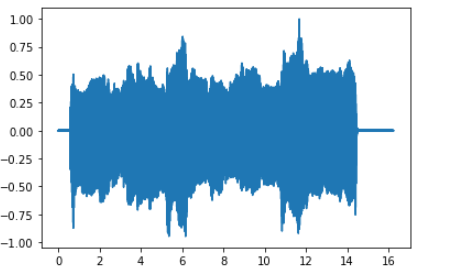
\includegraphics[width=0.75\textwidth]{2_1.png}
	\caption{Записанный звук}
	\label{fig:2.1}
\end{figure}

Затем я выделил полусекундный сегмент
\begin{lstlisting}[caption=Сегмент и его прослушивание]
	segment = wave.segment(start=1.0, duration=0.5)
	segment.make_audio()
\end{lstlisting}

И визуализировал его
\begin{lstlisting}[caption=Визуализация сегмента]
	segment.plot()
\end{lstlisting}

\begin{figure}[H]
	\centering
	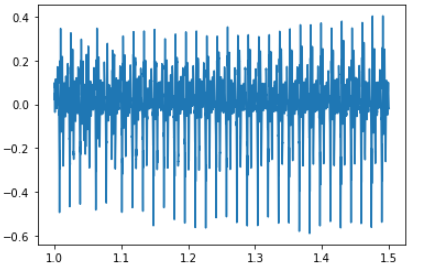
\includegraphics[width=0.75\textwidth]{2_2.png}
	\caption{Сегмент}
	\label{fig:2.2}
\end{figure}

\begin{lstlisting}[caption=Фрагмент сегмента]
	segment.segment(start=1.1, duration=0.01).plot()
\end{lstlisting}

\begin{figure}[H]
	\centering
	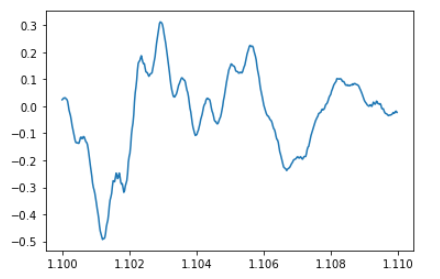
\includegraphics[width=0.75\textwidth]{2_3.png}
	\caption{Фрагмент сегмента}
	\label{fig:2.3}
\end{figure}

Затем я выделил спектр сегмента
\begin{lstlisting}[caption=Спектр сегмента]
	spectrum = segment.make_spectrum()
	spectrum.plot(high=7000)
\end{lstlisting}
\begin{figure}[H]
	\centering
	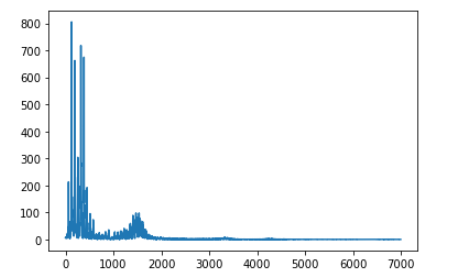
\includegraphics[width=0.75\textwidth]{2_4.png}
	\caption{Спектр сегмента}
	\label{fig:2.4}
\end{figure}
\begin{lstlisting}[caption=Основные и доминирующие частоты]
	spectrum = segment.make_spectrum()
	spectrum.plot(high=1000)
\end{lstlisting}
\begin{figure}[H]
	\centering
	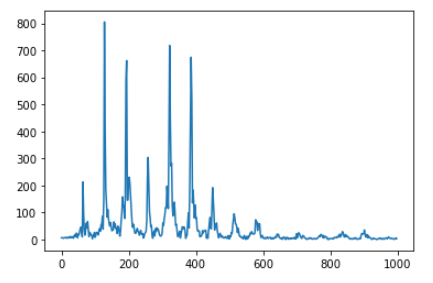
\includegraphics[width=0.75\textwidth]{2_5.png}
	\caption{Основные и доминирующие частоты}
	\label{fig:2.5}
\end{figure}
\end{enumerate}

Теперь выведем самые высокие точки спектра и их частоты в порядке 
убывания
\begin{lstlisting}[caption=Пики спектра]
	spectrum.peaks()[:30]
	
	[(805.2011660028415, 128.0),
	(717.7534137378161, 322.0),
	(674.4257107121337, 386.0),
	(662.1792673529742, 194.0),
	(590.2975588029225, 192.0),
	(522.1861101938315, 388.0),
	(452.49523817628216, 324.0),
	(451.2926648076347, 384.0),
	(401.46804683039875, 130.0),
	(386.27598232673955, 320.0),
	(304.0156833122087, 258.0),
	(282.4848989689322, 328.0),
	(272.01525283371285, 326.0),
	(230.78182369574293, 202.0),
	(229.5602546915074, 256.0),
	(222.41384500322584, 200.0),
	(213.0448913102804, 64.0),
	(203.73496641597413, 204.0),
	(203.0809167531178, 260.0),
	(199.3804441543911, 382.0),
	(197.24287528975682, 314.0),
	(192.08672045960517, 450.0),
	(187.7791701290673, 132.0),
	(182.9641942180879, 392.0),
	(167.77207719800455, 316.0),
	(160.52351987778476, 190.0),
	(158.17239516488624, 182.0),
	(155.35505888892268, 206.0),
	(151.3961428346756, 126.0),
	(150.398009639692, 452.0)]
\end{lstlisting}


Теперь отфильтруем гармоники
\begin{lstlisting}[caption=Фильтрация гармоник: low\_pass]
	spectrum.low_pass(2000)
	spectrum.make_wave().make_audio()
	
	spectrum.make_wave().plot()
\end{lstlisting}
\begin{figure}[H]
	\centering
	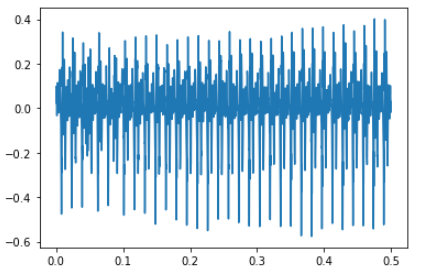
\includegraphics[width=0.75\textwidth]{2_6.png}
	\caption{Фильтрация гармоник: low\_pass}
	\label{fig:2.6}
\end{figure}

Как видно из графика, звук поредел, а звучать он стал глухо, как-будто из-за стены.

\begin{lstlisting}[caption=Фильтрация гармоник: high\_pass]
	spectrum.high_pass(2000)
	spectrum.make_wave().make_audio()
	
	spectrum.make_wave().plot()
\end{lstlisting}
\begin{figure}[H]
	\centering
	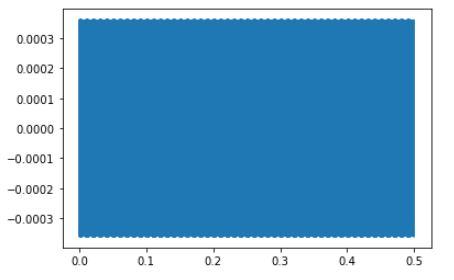
\includegraphics[width=0.75\textwidth]{2_7.png}
	\caption{Фильтрация гармоник: high\_pass}
	\label{fig:2.6}
\end{figure}

Звук стал похож на высокочастотный писк, как у звукового сигнала перед записью сообщения на автооответчик на телефоне.

\section{Упражнение 1.3}

\begin{enumerate}

\item \textbf{Задание}

		Создайте сложный сигнал из объектов \textit{SinSignal} и \textit{CosSignal}, суммируя их. Обработайте сигнал для получения wave и прослушайте его. Вычислите \textit{Spectrum} и распечатайте. Что произойдет при добавлении частотных компонент, не кратных основным?

\item \textbf{Ход работы}

Создадим сложный сигнал
\begin{lstlisting}[caption=Сложный сигнал]
	from thinkdsp import SinSignal
	
	signal = (SinSignal(freq=300, amp=0.9) +
	SinSignal(freq=520, amp=2.0) +
	SinSignal(freq=750, amp=0.3))
	signal.plot()
\end{lstlisting}
\begin{figure}[H]
	\centering
	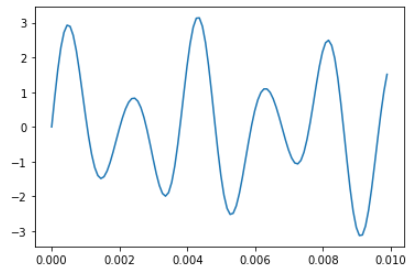
\includegraphics[width=0.75\textwidth]{3_1.png}
	\caption{Сложный сигнал}
	\label{fig:3.1}
\end{figure}

\begin{lstlisting}[caption=Прослушивание сложного сигнала]
	wave2 = signal.make_wave(duration=1)
	wave2.apodize()
	wave2.make_audio()
\end{lstlisting}

Звук похож на какую-нибудь низкую ноту, прозвучавщую из терменвокса.

Теперь вычислим спектр сложного сигнала
\begin{lstlisting}[caption=Спектр сложного сигнала]
	spectrum = wave2.make_spectrum()
	spectrum.plot(high=2000)
\end{lstlisting}
\begin{figure}[H]
	\centering
	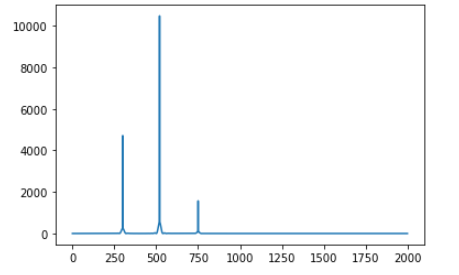
\includegraphics[width=0.75\textwidth]{3_2.png}
	\caption{Спектр сложного сигнала}
	\label{fig:3.2}
\end{figure}

Теперь добавим в звук новую частоту и прослушаем
\begin{lstlisting}[caption=Прослушивание спектра сложного сигнала]
	signal += SinSignal(freq=850)
	signal.make_wave().make_audio()
\end{lstlisting}
Звук стал выше (freq = 850). 

Теперь звук похож на какую-нибудь высокую ноту, прозвучавщую из терменвокса.

\end{enumerate}

\section{Упражнение 1.4}

\begin{enumerate}

\item \textbf{Задание}

		Напишите функцию \textit{stretch}, берущую wave и коэффициент изменения. Она должна ускорять или замедлять сигнал изменением \textit{ts} и \textit{framerate}. Подсказка: должно получиться всего две строки кода.

\item \textbf{Ход работы}

Напишем функцию \textbf{stretch} и прослушаем полученный результат
\begin{lstlisting}[caption=Функция stretch]
	wave3 = read_wave('res/throat_singing.wav')
	wave3.normalize()
	wave3.make_audio()
	
	def stretch(wave, factor):
	wave.ts *= factor
	wave.framerate /= factor
\end{lstlisting}

Попробуем замедлить звук
\begin{lstlisting}[caption=Замедленние звука]
	stretch(wave3, 1.5)
	wave3.make_audio()
\end{lstlisting}

Получился очень зловещий и низкий звук, как-будто какой-то огр недовольно мелодично рычит

Визуализируем результат
\begin{lstlisting}[caption=Визуализация замедленного звука]
	wave3.plot()
\end{lstlisting}
\begin{figure}[H]
	\centering
	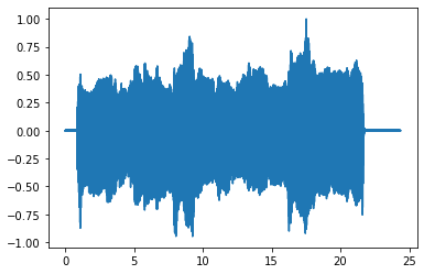
\includegraphics[width=0.75\textwidth]{4_1.png}
	\caption{Замедленный звук}
	\label{fig:4.1}
\end{figure}

Попробуем ускорить звук
\begin{lstlisting}[caption=Ускоренние звука]
	stretch(wave3, 0.5)
	wave3.make_audio()
\end{lstlisting}

Получился очень забавный высокий звук, как-будто какой-нибудь маленький тувинский мальчик осваивает горловое пение.

Визуализируем результат
\begin{lstlisting}[caption=Визуализация ускоренного звука]
	wave3.plot()
\end{lstlisting}
\begin{figure}[H]
	\centering
	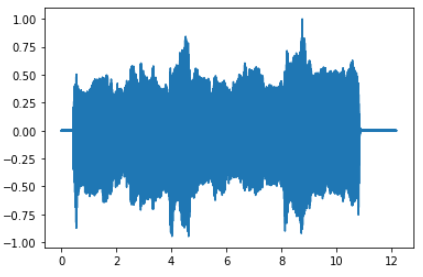
\includegraphics[width=0.75\textwidth]{4_2.png}
	\caption{Ускоренный звук}
	\label{fig:4.2}
\end{figure}

\end{enumerate}

\section{Вывод}

В результате выполнения лабораторной работы получены навыки работы со звуками: обработка, понижение/повышение частоты, вычисление пиков. Оказывается, работа со звуками очень занимательное и в какой-то мере забавное занятие, потому что всегда интересно послушать, что получится на выходе, в результате обработки.

\end{document}
